\section{Clamper Diode Circuit}

Các mạch trong hình bên dưới được gọi là bộ kẹp hoặc bộ phục hồi DC. Mô phỏng trên PSpice cũng được hiển thị trong hình bên dưới. Các mạch này kẹp một đỉnh của dạng sóng ở mức DC cụ thể (ví dụ: 0,7V). Học sinh được yêu cầu triển khai mạch trong PSPice để xác minh kết quả của họ từ tính toán lý thuyết.

\begin{figure}[h]
    \centering
    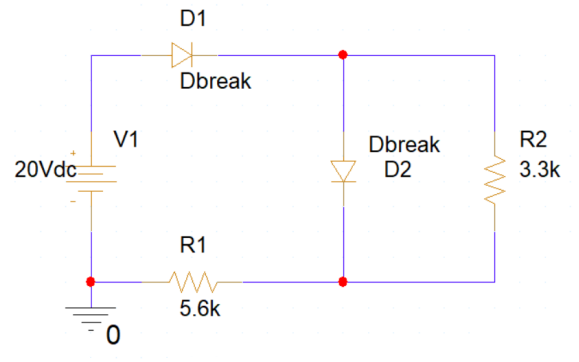
\includegraphics[width=0.5\textwidth]{graphics/ex4/f1.PNG}
    \caption{Mạch kẹp sử dụng Diode}
\end{figure}

\subsection{Tính toán lý thuyết}

Trong phần này, giả định rằng mô hình diode thực tế được sử dụng. Trình bày các phương trình của bạn để tính toán ba dòng điện khác nhau, bao gồm $I_{R1}, I_{R2}, I_{D2}$ và điện áp $V_{R2}$.

Theo Kirchhoff’s Voltage Law (KVL), ta có hai phương trình sau:
\begin{align}
    &E - V_{D1} - V_{D2} - 5.6 \cdot I_{R1} = 0 \\
    &V_{D2} = 3.3 \cdot I_{R2}
\end{align}
Theo Kirchhoff’s Current Law (KCL), ta có:
\begin{align}
    I_{R1} &= I_{R2} + I_{D2}
\end{align}

Từ (3.1), (3.2) và (3.3), ta có:
\begin{align*}
    &I_{R1} = 3,321 \, \text{mA} \\
    &I_{R2} = 0,212 \, \text{mA} \\
    &I_{D2} = 3,109 \, \text{mA} \\
    &V_{R2} = V_{D2} = 0.7 \, \text{V}
\end{align*}

\subsection{Mô phỏng PSpice}

Mô phỏng bias point được chạy trong PSpice. Chụp màn hình của bạn với điện áp và dòng điện được bật trong kết quả.

\begin{figure}[h]
    \centering
    \begin{subfigure}{0.49\textwidth}
        \centering
        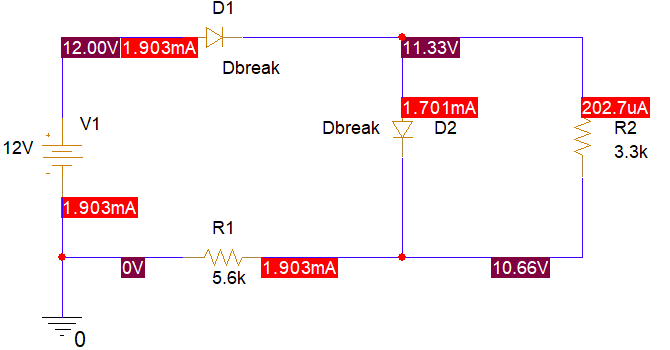
\includegraphics[width=\linewidth]{graphics/ex4/f2.PNG}
    \end{subfigure}
    \hfill
    \begin{subfigure}{0.49\textwidth}
        \centering
        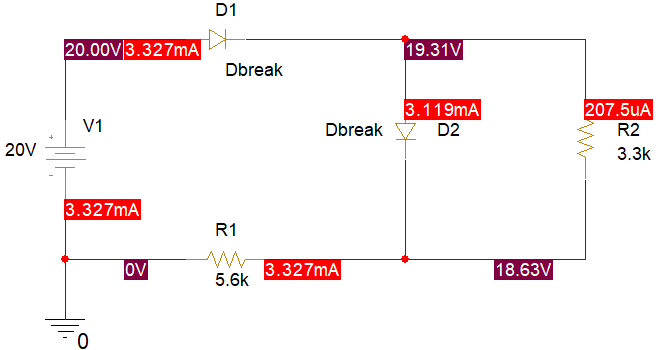
\includegraphics[width=\linewidth]{graphics/ex4/f3.PNG}
    \end{subfigure}
    \caption{Kết quả mô phỏng trên PSpice}
\end{figure}

\subsection{So sánh}

Sinh viên phải tóm tắt kết quả từ cả tính toán lý thuyết và mô phỏng PSpice và điền vào bảng bên dưới.

\begin{table}[h]
    \centering
    \begin{tabular}{@{}lcccccccc@{}}
        \toprule
        & \multicolumn{4}{c}{\textbf{Theory calculation}} & \multicolumn{4}{c}{\textbf{PSpice simulation}} \\

        \cmidrule(rl{0.5cm}){2-5} \cmidrule(rl{0.5cm}){6-9}

        & \makecell{\(I_{R1}\) \\(mA)} & \makecell{\(I_{R2}\) \\ (mA)} & \makecell{\(I_{D2}\) \\ (mA)} & \makecell{\(V_{R2}\) \\ (V)} & \makecell{\(I_{R1}\) \\ (mA)} & \makecell{\(I_{R2}\) \\ (mA)} & \makecell{\(I_{D2}\) \\ (mA)} & \makecell{\(V_{R2}\) \\ (V)} \\

        \midrule

        \(V\) = 12V & 1.893 & 0.212 & 1.681 & 0.70 & 1.903 & 0.203 & 1.701 & 0.67 \\
        \(V\) = 20V & 3.321 & 0.212 & 3.109 & 0.70 & 3.327 & 0.208 & 3.119 & 0.68 \\

        \bottomrule
    \end{tabular}
\end{table}

\textbf{Kết luận:} Chúng ta có thể thấy rằng với mạch này, trong mô hình Practical diode, diode D2 cố định điện áp và dòng điện qua R2, ở mọi giá trị của V. Ngược lại, trong mô phỏng Pspice, do điện trở nội bên trong Diode không phải là hằng số nên hai giá trị trên có sự khác nhau ở hai trường hợp.